% !TEX TS-program = xelatex
% !TEX encoding = UTF-8 Unicode

\providecommand{\home}{../..}
\documentclass[\home/main.tex]{subfiles}

\begin{document}

\graphicspath{{\home/figures}}

\chapter{Robotic folding in simulation}\label{ch:simulation}

% https://ieeexplore.ieee.org/stamp/stamp.jsp?tp=&arnumber=9386154

In this chapter, we explore the use of simulation for training robotic controllers for deformable object manipulation. We frame the usage of and the difference between robotics simulators and physics simulator. We compare different simulation technologies and implementations, and finally discuss results on learning to fold in simulation. 

\section{Digital twins}

% Why use simulation: rise of virtual env "digital twin"
Using a digital representation of a robot and the environment in which it operates allows reducing costly time on the real robot. This use-case has given rise to the term \emph{digital twin} meaning that the physical platform has a virtual representation which can be utilized. This digital twin is a cost-effective tool for for learning and safe experimentation. These benefits have proven their merit in the robotics field which has led to a plethora of simulator choices available to researchers \autocite{Collins2021}. However, navigating the simulation landscape is difficult and requires pinpointing exact requirements. For the research executed in this dissertation we require a simulation tool able to simulate robots and the associated physics, simulate cloth and can communicate with the physical robot. An additional bonus is the ease in which the simulation environment can be interfaced with off-the-shelf machine learning and reinforcement learning libraries that often require a Python interpreter. 
We discuss these requirements and constraints in the following sections. 

Figuur: venn diagram? 
We functionally distinguish X components: 
    which rigid body simulator can be used
    Which robotics simulation environment can be used and which functionalities does it expose 
    soft body simulation 
rigid body modeling with robotics support, soft body simulation

% What do we need: our use-case 

\section{Robotic simulation {\tiny pybullet, gazebo, nvidia, v-rep, unity. Nadruk op Unity en motivatie.}}

% What is a robot simulator and how does it differ from physics simulator. Also real integrations: URDF, ROS communication with real robot. 
A robot simulator encapsulates a physics engine while exposing other functionalities. This is an important distinction between physics and robotic simulations. The former is a part of robotic simulation and provides realistic modelling and simulation of physical phenomena. The physics engine handles the construction and articulation of kinematic chains, querying collision detection, providing friction models and optionally has built-in soft body support. 
% Robot vs physics simulation
In \cref{sec:lit_simulation}, we discussed two categories of physics engines: real-time and offline. For robotic learning purposes, we prioritize simulation speed above accuracy so we only consider real-time physic engines. There is a wide variety of real-time physics simulators available such as Bullet \autocite{Bullet}, PhysX \autocite{PhysX}, Havok \autocite{Havok}, ODE \autocite{ODE} and MuJoCo \autocite{Mujoco}. 
% Problem with many physics engines: cartesian instead of joint representation
With the exception of MuJoCo, these physics engines are primarily developed for gaming purposes that require real-time simulation. However, in gaming and visualization applications, most bodies have few or even none joints or constraints. Consequently, many physics engines model physical bodies with a Cartesian representation in which each rigid body has 6 degrees of freedom. The joints of a body then becomes constraints imposed on the $6N$-dimensional space. This is in contrast to robots that are multi-body systems of $N$ constrainted links that makes the system dimensionality much closer to $N$ instead of $6N$. Hence, we have a strong preference for robotic simulators that have underlying physic engines using generalized joint coordinates that provide better stability, speed and accuracy. The difference between generalized coordinates versus Cartesian coordinates representation is illustrated in \cref{fig:generalized_vs_cartesian_coordinates}. This example demonstrates that a double pendulum can be represented as a 12 degrees of freedom system with 10 constraints or as a 2 degrees of freedom system without constraints. 

\begin{figure}
    \centering
    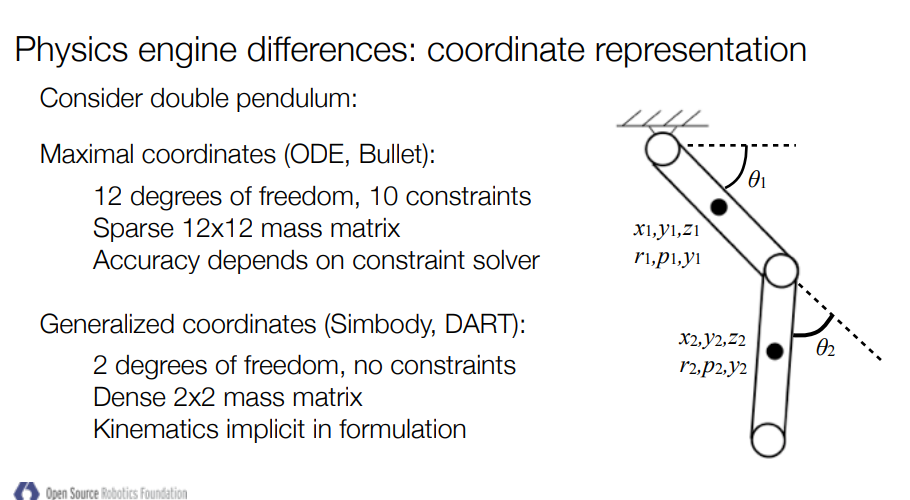
\includegraphics[]{figures/gen_vs_max_coordinates.png}
    \caption[Comparison between generalized and Cartesian coordinates for representing multibody kinematic chains.]{\textbf{Comparison between generalized and Cartesian coordinates for representing multibody kinematic chains.} A double pendulum can be represented as two links each having 6 degrees of freedom: 3 possible translations and 3 possible rotations. In this Cartesian representation, all translations and 2 rotations are constrained per link. The joint coordinate however, represents the system with 2 degrees of freedom $\theta_1$ and $\theta_2$ with no constraints. TODO: make own fig. }
    \label{fig:generalized_vs_cartesian_coordinates}
\end{figure}

% Other robotic simulator functionality
On top of integrating a physics simulation, the robotic simulator exposes functionality specific to the robotics domain.
% URDF
One of these features is importing predescriped robot models that are often expressed in Unified Robot Description Format\footnote{\url{http://wiki.ros.org/urdf}}. 
% Actuators, control modes
The simulator must provide actuator models for position control, velocity control, and torque control in order to control the physical arms. 
% IK, FK
Forward kinematics and inverse kinematics are needed for path planning functionality. 
% Sensors
Robots for manipulation tasks are equipped with various sensors such as RGB-D cameras, torque and force sensors which need to be supported by the simulator as well. 
% Rendering
Similarly to RGB-D cameras, the simulator benefits from having a rendering pipeline for visualization and debugging purposes. This rendering pipeline can be used as RGB-D camera and preferably is able to execute headless for server-side rendering.  
% ROS
In order for the digital twin to communicate with its physical counterpart, it needs messaging channels to the real platform. The communication is often provided through ROS\footnote{\url{https://www.ros.org}}; a middleware software suit providing hardware abstraction through message-passing nodes. 

% Short comparison of robot simulation technologies
In this research, we compared the following robotic simulators: PyBullet \autocite{pybullet}, MuJoCo\texttrademark, Gazebo and Unity\texttrademark \autocite{Unity}. The goal of this chapter is not to provide an exhaustive comparison between popular robotics simulators for manipulation tasks. A thorough comparison would require setting up multiple scenarios, relevant metrics and experience with the simulation technology. For example, it is unclear whether we should compare accuracy, scalability, stability, speed or performance in the context of the robotic manipulation tasks, which also depends on the used controller. \textcite{Giovanni2011} for example, found that the simulation engine does not matter when using robust controllers for generating gaits. It is hard to concretely measure such metrics. For example, accuracy is difficult to quantify in the absence of analytical solutions.
Given that all robotic simulators at the time did not provide adequate cloth simulation support, we instead performed a qualitative tradeoff, consulted the documentation, forums and the limited amount of literature available at the time comparing the simulators \autocite{staranowicz2011survey,Erez2015}.

PyBullet is a framework written in the Python programming language on top of the Bullet physics engine. It provides robot functionality with Python bindings. PyBullet has a focus on machine learning in robotics. At time of executing this research, PyBullet was recently introduced and a one-man effort making the implementation immature. Many features needed yet to be implemented or were not exposed to the Python API. In addition, Bullet recently switched from Cartesian to joint coordinates representation which was not thoroughly debugged. Compared to main-stream game engines, the rendering capabilities of PyBullet are subpar. Finally, PyBullet provides an experimental soft body implementation which we, among other authors \autocite{Matas2018, seita2021learning}, found unuseable. The soft body physics caused cloth to tunnel or explode on grasping attempts and only wireframe rendering was possible at the time. 

Gazebo is an open-source robotics simulation environment supported by ROS. It exposes multiple physics engines, most notably Bullet and ODE. The Bullet physics engine suffers from the above mentioned shortcomings while ODE only offers Cartesian multibody representation, making it slow and stable for robotics. Gazebo is strongly integrated with the ROS ecosystem, making it very feature-complete for transfer to real robots. The physics engine underpinning Gazebo do not offer cloth simulation.

Mujoco is blablabl. MuJoCo is generally known for its stable and efficient multibody system dynamics\autocite{Erez2015}.
At time of executing our research, MuJoCo required a license which made does not fit for our purposes to be able to run simulations on remote servers. 
MuJoCo supports most of the features mentioned at the start of this section but lacks support for inverse
kinematics and path planning.
MuJoCo provides volumetric soft body simulation of which the generalization towards planar soft bodies is unclear. 

Unity is balbalb. 


\begin{table}[]
    \begin{tabular}{lllll}
                    & PyBullet & MuJoCo & Gazebo & Unity \\
    Stable physics  &     yes     &  yes      &    yes    &  yes     \\
    URDF support    &      yes    &    yes    &    yes    &   yes    \\
    Coordinates     &  Minimal &  Minimal  & Minimal \& Cartesian       & Minimal \& Cartesian    \\
    Python bindings &    yes      &   limited via community     &    yes    &   yes   \\
    Rendering       &    -     &   ++     &   +     & +++ \\     
    Soft body support       &    nonfunctional     &   limited     &   no     & nonfunctional \\     

    \end{tabular}
    \caption{Note }
\end{table}

% why do we go for Unity
Ultimately, we decided that Unity is the best: good IDE, broad community and corporative support, incumbent player in robotics, ease-of-use for extending physics simulations for cloth, high-quality rendering and recent changes for providing minimal joint coordinates simulation and solver. 

\section{Cloth simulation \tiny{particle system, msd, integrator , ...} }
% OP REIS TODO: schrijf particle simulation gedeelte. Lees eerst de typische papers voor structuur maar gebruik uiteindelijk muller zijn notes. 

%Zie ook "Robotic manipulation and sensing of deformable objects in domestic and industrial applications: a survey" p4 voor overzicht om te introduceren maar focus op particle based methods.
%  zie ook Dexterous Robotic Manipulation of Deformable Objects with Multi-Sensory Feedback - a Review van khalil
% background sectie 3 van SoftGym": https://arxiv.org/pdf/2011.07215.pdf
%  Voor de specifieke methode, zie ook p47 van Seita zijn boek 
%  Zie ook Muller notes about deformable object manipulation p11



\section{Learning to fold in simulation}
% hier moet ik nog wat nadenken over het doel van deze sectie 
% het demonstreren dat de simulator werkt, dat plooien kan 
% tonen dat DRL werkt maar veel iteraties nodig heeft. De reward functie is godmode en moeilijk te transfereren naar het echt 
% eventueel een behavioral cloning approach ook tonen. Dan showcasen waar het zich vastrijdt
% eventueel iets over sim2real problemen dat hier al naar boven komen 
\subsection{Deep reinforcement learning setup for cloth folding in simulation}
\subsection{Results \tiny{om te tonen dat leren mogelijk is in deze setup maar wat de moeilijkheden zijn: de reward, godmode en aantal obs}}

\footnote{The implementation of the simulation is developed in context of a software engineering course with students }


\section{Conclusion {\tiny considerations, approaches, our approach, DRL works but reward function godmode and many iterations}}

\end{document}